\section{Parallele Realisierung}
Nachdem die serielle Implementierung zufriedenstellende Ergebnisse lieferte, konnten wir uns dem übergeordneten Ziel widmen unser 
Programm zu parallelisieren.\newline
Strukturell besteht ein Pythagoras-Baum aus einer Menge von Daten --- in unserem Fall Cuboid-Objekten ---
auf die immer wieder dieselbe Operation angewendet wird. Es handelt sich also um eine Datenparallelität. Aufgrund der linearen Speicherung
in einem Array beziehungsweise einem Vektor benötigen wir nur eine Dimension.\newline
Zwischen den Quadern einer Ebene bestehen keinerlei Abhängigkeiten. Dementsprechend ist eine Kommunikation oder Synchronisierung zwischen den einzelnen
Berechnungseinheiten generell nicht notwendig. 

\subsection{OpenCL}
\vspace{-0.25cm}
Unser erster Schritt war die Parallelisierung unter Verwendung der GPU. Da nur einer der verwendeten Laptops (Thinkpad P15) über eine 
Nvidia-Grafikkarte verfügte, fiel unsere Wahl auf OpenCL als Schnittstelle.\\
Grundsätzlich konnten wir eine zu unserer seriellen iterativen Funktion äquivalente Lösung implementieren --- es waren jedoch umfassende
Änderungen in unserem Programm notwendig. Da OpenCL reinen C-Code statt des bisher verwendeten C++ benötigte, mussten alle geschriebenen
C++-Klassen in C-Structs umgewandelt werden. In den für OpenCL relevanten Funktionen mussten wir außerdem auf den Einsatz von Funktionen
aus der C++ Standardbibliothek verzichten. \\
Eine zusätzliche Herausforderung war, dass alle im OpenCL-Kernel genutzten Funktionen direkt in der kernel.cl implementiert werden
mussten, wodurch eine große und unübersichtliche Datei entstand. 

\vspace{0.25cm}
Ähnlich wie bei der sequentiellen Version implementierten wir auch für die Umsetzung mit OpenCL eine Funktion 
\lstinline{generateWithOpenCL()}. Diese ruft die verfügbaren OpenCL Plattformen und Geräte ab und wählt die GPU als OpenCL device aus. 
Daraufhin wird ein Kontext und eine Command Queue erstellt, bevor der OpenCL-Kernel aus der kernel.cl eingelesen und kompiliert
wird. \\
Für die Berechnung der für den Baum benötigten Quader auf der GPU entschieden wir uns für einen feingranularen Ansatz, bei
welchem jeder Thread für genau einen Quader zuständig ist. Resultierend daraus war die Anzahl der benötigten GPU-Threads nicht vorab
festlegbar, weil sie sich mit jeder Ebene verdoppelte.
Grundsätzlich wäre eine feinere Granulierung möglich, indem beispielsweise
jeder Thread die Transformation eines einzelnen Punktes vornimmt --- hierbei wäre jedoch der Aufwand, die Daten sinnvoll zu verteilen
und anschließend korrekt wieder zusammenzufügen, exponentiell höher.\\
Zur Übermittlung des Vektors mit den bereits vorhandenen Quadern an die GPU und zum Zurückliefern des Arrays mit den erzeugten Quadern
nach Vollendung der Berechnungen an die CPU implementierten wir ein Double-Buffering-System\footnote{Double-Buffering = Verwendung 
zweier Buffer, die abwechselnd gefüllt werden, um Verzögerungen durch das Leeren und Löschen von Daten zu vermeiden}. 
Die Buffer werden vor dem Aufruf des Kernelcodes in unserer \lstinline{generateWithOpenCL()}-Funktion angelegt und auf die GPU übertragen. 

\subsubsection*{Näherungsfunktionen auf der GPU}
\vspace{-0.25cm}
Wie wir in der Vorlesung gelernt haben, haben Näherungsfunktionen wie Potenzen, Wurzeln oder auch trigonometrische Funktionen einen
negativen Einfluss auf die Performance von auf der GPU ausgeführten Programmen. Im Pythagoras-Baum kommen nicht nur Potenzen (welche
im benötigten Rahmen problemlos durch Multiplikationen ersetzbar waren) und Wurzeln, sondern vor allem auch Sinus- und Cosinusberechnungen 
zum Einsatz.\\
Initial planten wir, eine Sinus-Lookup-Table auf der CPU zu erstellen und diese als Buffer an die GPU zu übergeben. Unsere Recherche ergab
jedoch, dass dieser Ansatz auf der GPU bereits umgesetzt wird. Stattdessen wird die Verwendung von \texttt{native\_sin()} und
\texttt{native\_cos()} empfohlen. Die \glqq native\grqq-Funktionen liefern Näherungen mit für unsere Zwecke akzeptabler Genauigkeit und benötigen
maßgeblich weniger Laufzeit als die herkömmlichen \texttt{sin()}- und \texttt{cos()}-Funktionen.\footnote{Quellen (letzter Zugriff: 03.02.2026): 
\href{https://stackoverflow.com/questions/62546207/how-to-optimize-opencl-kernel-use-of-trigonometric-functions}{Stackoverflow - How to optimize OpenCL-Kernel use of trigonometric funktions} /
\href{https://registry.khronos.org/OpenCL/sdk/3.0/docs/man/html/erf.html}{khronos.org - OpenCL docs} /
\href{https://developer.download.nvidia.com/compute/DevZone/docs/html/OpenCL/doc/OpenCL_Best_Practices_Guide.pdf}{nvidia.com - OpenCL Best Practices Guide}}
Ein Nachteil dieses Ansatzes liegt in der limitierten Verfügbarkeit --- die \texttt{native}-Funktionen sind nicht auf allen
Rechnern respektive nicht bei allen OpenCL-Implementierungen verfügbar.\\
Darüber hinaus reduzierten wir die Menge der trigonometrischen Berechnungen, indem wir die Sinus- und Cosinus-Werte
für die Berechnung der Punkt-Transformation einmalig zu Beginn der Funktion berechneten, statt sie mehrfach neu zu kalkulieren. 
Auf einem Rechner mit Nvidia-GPU erreichten wir so eine Beschleunigung von bis zu 40\%. 
% https://stackoverflow.com/questions/62546207/how-to-optimize-opencl-kernel-use-of-trigonometric-functions

% https://registry.khronos.org/OpenCL/sdk/3.0/docs/man/html/erf.html
% A subset of functions from Built-in Scalar and Vector Argument Math Functions that are defined 
% with the native_ prefix. These functions may map to one or more native device instructions and 
% will typically have better performance compared to the corresponding functions without the native_ prefix). 
% The accuracy (and in some cases the input range(s)) of these functions is implementation-defined.

% https://developer.download.nvidia.com/compute/DevZone/docs/html/OpenCL/doc/OpenCL_Best_Practices_Guide.pdf
% Two types of runtime math operations are supported. They are
% native_functionName() and functionName(). Functions using
% native_functionName() map directly to the hardware level. They are faster but
% provide somewhat lower accuracy. (Examples: native_sin(x), native_exp(x),
% and so forth.) Functions using functionName() are slower but have higher
% accuracy. (Examples: sin(x), exp(x), and so forth.) The throughput of
% native_sin(x), native_cos(x), native_exp(x) is 1 operation per clock cycle,
% while sin(x), cos(x), tan(x) are much more expensive and become even more so
% (about an order of magnitude slower) if the absolute value of x needs to be reduced.
% Moreover, in such cases, the argument-reduction code uses local memory, which
% can affect performance even more because of the high latency of local memory.
% More details are available in the NVIDIA OpenCL Programming Guide.

% NOCH NICHT GELESEN ABER EVENTUELL LESENSWERT: 
% https://ijecce.org/administrator/components/com_jresearch/files/publications/IJECCE-3291_Final.pdf

\vspace{-0.25cm}
\subsubsection*{Zufallsbäume auf der GPU}
\vspace{-0.25cm}
Die Verwendung von Funktionen aus der C++ Standardbibliothek ist in OpenCL nicht möglich 
und das Erzeugen von Zufallszahlen auf der GPU generell problematisch. Daher mussten wir für das Generieren
zufälliger Bäume mit OpenCL die Zufallszahlen vorab auf der CPU erzeugen und an die GPU übergeben.\\
Glücklicherweise ließ sich die hierfür aufzubringende Zeit einfach minimieren, indem wir nur eine kleine Menge
Zahlen kalkulierten, die im Laufe der Berechnungen auf der GPU wiederverwendet werden konnten.
Theoretisch wäre eine Primzahl als Menge von Zufallszahlen vermutlich optimal. Wir erzielten jedoch auch mit 42 
Zufallszahlen schon Ergebnisse, die visuell einen guten Eindruck von Zufälligkeit erweckten. 
\vspace{0.5cm}\\
\begin{minipage}{0.49\linewidth}
   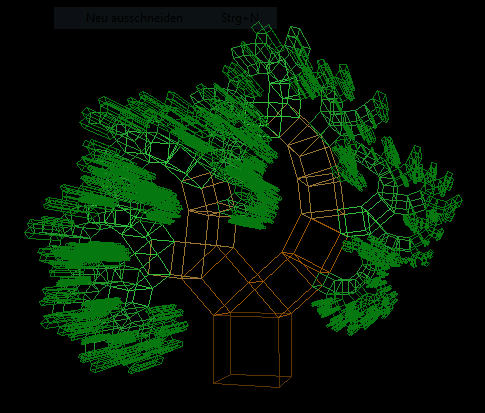
\includegraphics[width=\linewidth]{pictures/OCL_random_Depth10.PNG}
   \captionof{figure}{Zufallsbaum mit 10 Ebenen generiert auf der GPU}
   \label{fig:GPU-Rand-1}
\end{minipage}
\hfill
\begin{minipage}{0.49\linewidth}
   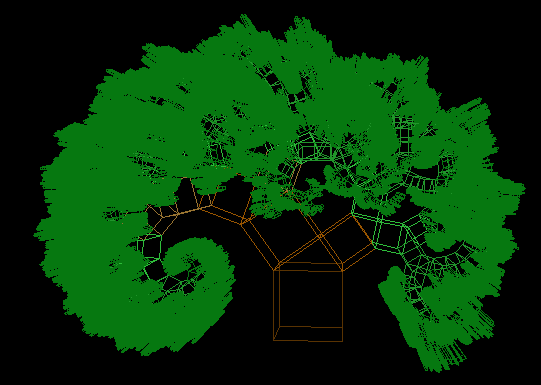
\includegraphics[width=\linewidth]{pictures/OCL_random_Depth18.PNG}
   \captionof{figure}{Zufallsbaum mit 18 Ebenen generiert auf der GPU}
   \label{fig:GPU-Rand-2}
\end{minipage}

% ----------------------------------- OpenMP ---------------------------------------
% ----------------------------------------------------------------------------------
\subsection{OpenMP}
\subsubsection*{Erzeugung einer Sinus-Lookup-Tabelle}
\vspace{-0.25cm}
Aufgrund der bekannten Problematik der Ineffizienz trigonometrischer Funktionen auf der GPU kam uns schon in der Planungsphase
unseres Projekts die Idee, mit OpenMP eine Sinus-Lookup-Tabelle zu berechnen. Diese sollte als Buffer auf die GPU übertragen
und dort bei den Berechnungen des \hyperref[Sinussatz]{Sinussatzes} und der Transformationsmatrizen verwendet werden.
Bevor wir feststellten, dass die GPU intern eine derartige Optimierung bereits verwendet, hatten wir eine erste Version dieses 
Ansatzes bereits implementiert. Dabei mussten wir jedoch feststellen, dass schon das sequentielle Befüllen des Arrays so schnell war,
dass eine Parallelisierung keinen Mehrwert geboten hätte.\\
Letztendlich entschieden wir uns dagegen, diese Idee weiter zu verfolgen.

\subsubsection*{Erzeugen von Pythagoras-Bäumen}
\vspace{-0.25cm}
Auch die mit OpenMP parallelisierte Implementierung in der Funktion \lstinline{generateWithOpenMP()} folgt demselben Konzept wie die sequentielle
iterative Funktion. Anders als für die Umsetzung von OpenCL mussten hierfür keine umfassenden Änderungen unseres Programms erfolgen. Da wir zur
iterativen Erstellung der Pythagoras-Bäume mit for-Schleifen arbeiten, konnten wir zur Parallelisierung das Pragma
\lstinline{#pragma omp parallel for} verwenden.\\
Um beim Sammeln der berechneten Quader im Result-Vektor keine Daten zu verlieren, arbeiteten wir anfangs mit einem kritischen Bereich. Diesen 
konnten wir durch Verwenden der durch die Laufvariable der for-Schleife vorgegebenen Indizes entfernen:
\vspace{0.25cm}\\
\begin{minipage}{0.58\linewidth}
\begin{lstlisting}[caption={Ausschnitt generateWithOpenMP(): Kritischer Bereich}]
...
 #pragma omp critical
 {
     resultCuboids.push_back(newCuboid_b);
     resultCuboids.push_back(newCuboid_a);
 }
...
\end{lstlisting}
\end{minipage}
\hfill
\begin{minipage}{0.35\linewidth}
\begin{lstlisting}[caption={Ersatz für kritischen Bereichs\\ i: Laufvariable for-Schleife}]
...
 resultCuboids[i*2+1] = newCuboid_b;
 resultCuboids[i*2] = newCuboid_a;
...
\end{lstlisting}
\end{minipage}
\vspace{0.25cm}\\
Das Generieren von Zufallsbäumen unter Nutzung von OpenMP stellte kein Problem dar. Ebenso wie in der sequentiellen Umsetzung konnte 
die \texttt{rand()}-Funktion aus der C++-Bibliothek eingesetzt werden.
\vspace{0.25cm}\\
Da auf der CPU in der Regel maximal acht oder 16 Kerne zur Verfügung stehen, ist die Parallelität hier deutlich grobgranularer als bei 
der GPU-Parallelisierung. Zwar verarbeiten wir nach wie vor jeden Quader einzeln, jedoch muss jeder CPU-Kern dabei eine große Menge Quader 
nacheinander berechnen. 

\begin{minipage}{0.49\linewidth}
   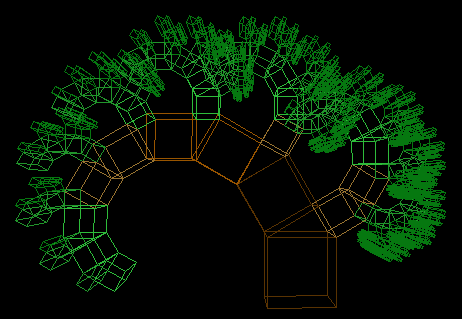
\includegraphics[width=\linewidth]{pictures/OMP_fixed_Depth8.PNG}
   \captionof{figure}{Pythagoras-Baum mit 8 Ebenen generiert mit OpenMP}
   \label{fig:OMP-fixed}
\end{minipage}
\hfill
\begin{minipage}{0.49\linewidth}
   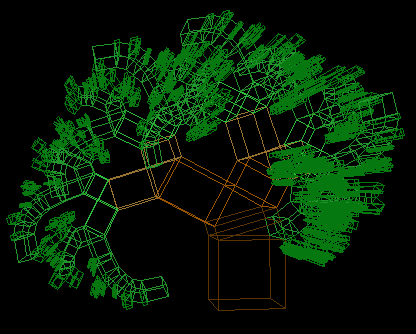
\includegraphics[width=\linewidth]{pictures/OMP_random_Depth10.PNG}
   \captionof{figure}{Zufallsbaum mit 10 Ebenen generiert mit OpenMP}
   \label{fig:OMP-random}
\end{minipage}

\subsubsection*{Hinzufügen von Objekten zum Renderer}\label{3-2-rendering}
\vspace{-0.25cm}
Die Quader des Pythagoras-Baums liegen nach ihrer Berechnung mit einer beliebigen Methode als Vektor vor und müssen einzeln
für den Renderer aufbereitet werden. Zwischen den verschiedenen Körpern bestehen keine Abhängigkeiten, sodass die umschließende for-Schleife
gut auf der CPU zu parallelisieren ist. Der Aufruf der Funktion \lstinline{addCuboidToRenderer()} zum Hinzufügen von Objekten zum Renderer erfolgt 
also parallelisiert. Daraus resultiert, dass auch bei der mit OpenCL parallelisierten und am Ende der sequentiellen Ausführung OpenMP zum Einsatz 
kommt, um die Gesamtlaufzeit des Programms zu verbessern.\\
Damit beim tatsächlichen Zugriff auf die Sammlung an Render-Objekten im Renderer Kollisionen verhindert werden, ist dieser separate Schritt als
kritischer Bereich markiert: 
\vspace{0.25cm}
\begin{lstlisting}[caption={Ausschnitt aus addCuboidToRenderer() mit kritischem Bereich}]
// Aufruf in main(): 
 #pragma omp parallel for
 for (Cuboid& c : cuboids) {
    addCuboidToRenderer(c, myRenderer);
 }

// Funktion: 
 void addCuboidToRenderer(const Cuboid &cube, Renderer& renderer) {
 ...
 #pragma omp critical
    renderer.addRenderObject(std::move(cubeObject));
 ...
 }
\end{lstlisting} 

% ----------------------------------- MPI ---------------------------------------
% -------------------------------------------------------------------------------
\newpage
\subsection{MPI}
\subsubsection{Konzeption}
\vspace{-0.25cm}
Analog zu den Implementierungen der bereits umgesetzen Funktionen sollte eine Funktion \lstinline{generateWithMPI()}
angelegt werden. Diese nimmt ein Inputarray mit mindestens einem Startquader sowie eine gewünschte Tiefe entgegen.\\
Zur parallelen Verarbeitung muss das Inputarray gleichmäßig auf die verfügbaren Rechner aufgeteilt werden. Prinzipiell kann
die Aufteilung da es keine Abhängigkeiten zwischen den Quadern gibt in n Sub-Arrays der Größe 
\[\frac{\text{Anzahl Inputquader}}{\text{Anzahl Prozesse}}
\quad \text{mit Anzahl Inputquader} = \text{inputarray.length()}
\]
erfolgen --- hierbei muss jedoch darauf geachtet werden, dass keine Quader übrig bleiben, wenn die Rechnung keine ganze Zahl ergibt. 
Anschließend kann jeder MPI-Prozess für seinen Teil der Inputquader die Folgequader berechnen.\\
Um nach Vollendung der Berechnungen wieder ein vollständiges Array mit allen Quadern zu erhalten, welches man an eine zentrale Instanz
zurückliefern kann, kann die MPI-Gather Methode zum Einsatz kommen.

\subsubsection{Umsetzung}
\vspace{-0.25cm}
Es ist zu erwarten, dass bei MPI dieselbe Problematik wie bei OpenCL durch das Umkopieren der Daten entstünde. Besonders dadurch, dass
der Transfer nicht länger innerhalb eines Rechners, sondern über das Netzwerk erfolgen müsste, gäbe es einen großen Overhead, der einen
Zeitgewinn unwahrscheinlich macht.\\
Darüber hinaus bliebe unser in \hyperref[Speicher]{Kapitel 5.4} detailliert aufgeführtes Speicherplatzproblem bestehen, weshalb 
eine Implementierung der MPI-Parallelisierung zum jetzigen Zeitpunkt keinen Mehrwert für die Laufzeit unseres Programms bieten kann.

% Chat-GPT:
% Overhead-Kosten:
%     MPI benötigt eine erhebliche Menge an overhead, um Prozesse zu starten und zu verwalten, was bei kleinen Datenmengen ineffizient sein kann.
% 
% Datenkommunikation:
%     Bei der Parallelisierung mit MPI wird die Kommunikation zwischen verteilten Prozessen über ein Netzwerk realisiert, was zusätzliche Latenzzeiten und Kommunikationsprobleme verursachen kann.
% 
% Anwendungsstruktur:
%     Der 3D Pythagorasbaum könnte in einer Einzel- oder Mehrkernumgebung effizienter umgesetzt werden, da die Datenlokalität und der Zugriff auf den gemeinsamen Speicher in einem Shared-Memory-System (wie bei OpenMP) besser unterstützt werden.
% 
% Einrichtungs- und Fehleraufwand:
%     MPI erfordert eine komplexere Setup- und Fehlerbehandlungslogik im Vergleich zu OpenCL und OpenMP, die in vielen Fällen nicht gerechtfertigt ist.
% 
% Keine signifikante Leistungsteigerung:
%     Wenn die zu verarbeitenden Daten oder die Berechnungen nicht ausreichend groß sind, kann MPI im Vergleich zu OpenCL oder OpenMP keine signifikante Leistungssteigerung bieten.
% 
% Portabilität und Zugänglichkeit:
%     Die Einführung von MPI könnte zusätzliche Anforderungen an die Hardware (z. B. mehrere Knoten oder Cluster) stellen, was die Portabilität und Zugänglichkeit für weniger erfahrene Benutzer einschränkt.
% 
% Eingeschränkte Parallelisierungsstrategien:
%     Da der Pythagorasbaum in einem rekursiven und hierarchischen Format data-parallelisiert wird, könnte die Verwendung von MPI zu einem Mangel an Flexibilität führen, da es primär für task-parallelistische Anwendungen konzipiert ist.

\subsection{Pattern und Operationen}
\vspace{-0.25cm}
Design-Pattern und vordefinierte Operationen helfen dabei, wiederkehrende programmatische Probleme bei der Parallelisierung eines Programms zu lösen.
Ein typisches Problem, auf welches wir während unserer Projektumsetzung stießen, war die ursprünglich rekursive sequentielle Funktion. Diese konnten
wir wie in \hyperref[iterativ]{Abschnitt 2.2} beschrieben unter Anwendung des Divide and Conquer Patterns\footnote{Divide and Conquer = Zerlegen eines Problems in Teilprobleme zur besseren Lösung} in eine 
iterative Version mit einer for-Schleife umwandeln. \\
Außerdem basiert die Generierung von Folgequadern aus den Inputquadern in unseren iterativen Umsetzungen auf einer Scatter-Operation. In jedem Schritt werden
aus einem eingelesenen Quader zwei Folgequader erzeugt.\\
Insgesamt tragen diese Strukturen dazu bei, die Komplexität des Codes zu reduzieren, die Last besser zu verteilen, die Skalierbarkeit zu erhöhen und so 
letztendlich die Laufzeit zu verbessern. 
